\chapter{Les polymères}\label{ch:g12:polymers}

Une veste polaire peut être filée à partir de bouteilles de boisson
fondues~; une corde d'escalade est en nylon~; cette page est faite de
cellulose, fabriquée par les arbres. Ce sont trois \omterm{def:g12:polymers:polymer}{polymères}~: des
\omterm{def:g7:atoms-and-molecules:molecule}{molécules} longues de milliers d'\omterm{def:g7:atoms-and-molecules:atom}{atomes}, construites en répétant encore
et encore un petit \omterm{def:g12:polymers:repeat-unit}{motif}. Leurs propriétés --- souples ou rigides,
élastiques ou cassants, fusibles ou non --- dépendent moins des \omterm{def:g7:atoms-and-molecules:atom}{atomes}
qu'ils contiennent que de la façon dont leurs longues chaînes sont
disposées.

\begin{recall}
Les \omterm{def:g8:plastics:plastic}{matières plastiques} sont faites de très longues \omterm{def:g7:atoms-and-molecules:molecule}{molécules}~; les
\omterm{def:g8:plastics:thermoplastic}{thermoplastiques} se ramollissent quand on les chauffe, les
\omterm{def:g8:plastics:thermoplastic}{thermodurcissables} non (\cref{ch:g8:plastics}). Les groupes \omterm{def:g11:functional-groups:alcohol}{alcool},
acide, \omterm{def:g11:functional-groups:carboxylic-acid}{ester}, \omterm{def:g11:functional-groups:amine}{amine} et \omterm{def:g11:functional-groups:amine}{amide} (\cref{ch:g11:functional-groups}). Une
\omterm{def:g12:curly-arrows:categories}{addition} réunit deux \omterm{def:g7:atoms-and-molecules:molecule}{molécules} en une seule sans perdre aucun \omterm{def:g7:atoms-and-molecules:atom}{atome}
(\cref{ch:g12:curly-arrows}).
\end{recall}

\begin{omfigure}
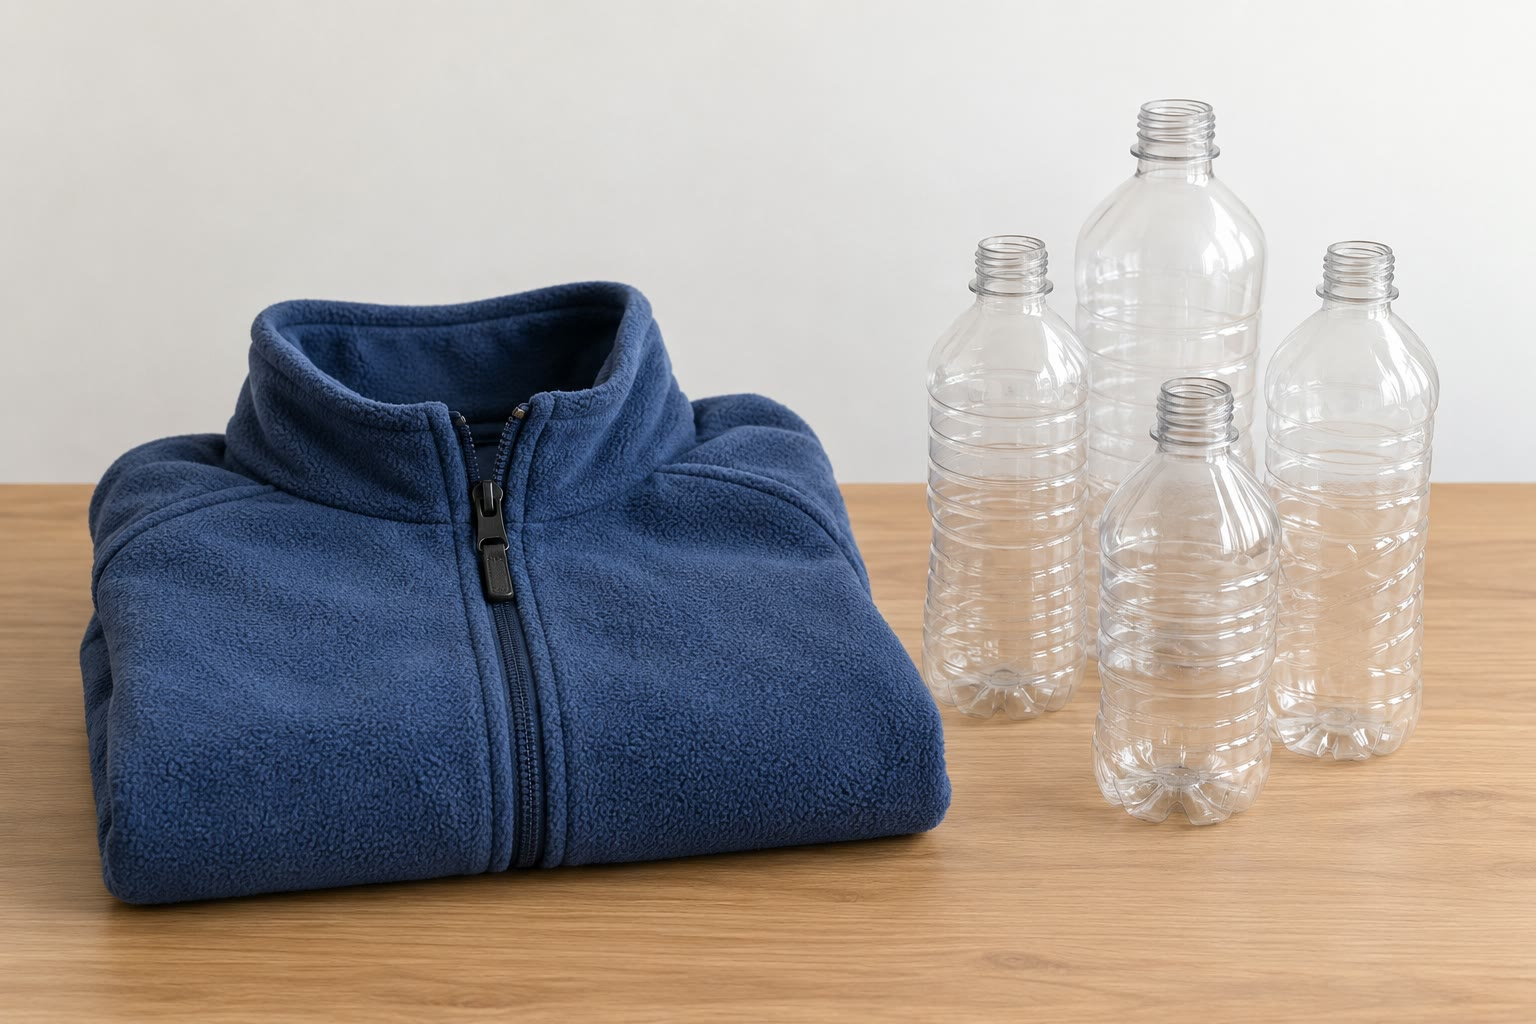
\includegraphics[width=0.45\linewidth]{images/book1/ai/g12-fleece-bottles.jpg}

{\small Des bouteilles de boisson usagées et une veste polaire~: le même
\omterm{def:g12:polymers:polymer}{polymère}, sous deux formes.}
\end{omfigure}

\section{Monomères, polymères, motifs}

\begin{definition}[Polymère, monomère, polymérisation]\label{def:g12:polymers:polymer}
Un \emph{polymère}\index{polymere@polymère} est une substance faite de très
grosses \omterm{def:g7:atoms-and-molecules:molecule}{molécules}, les macromolécules, construites chacune à partir de
nombreux petits \omterm{def:g12:polymers:repeat-unit}{motifs} liés les uns à la suite des autres. Les petites
\omterm{def:g7:atoms-and-molecules:molecule}{molécules} à partir desquelles il est fabriqué sont ses
\emph{monomères}\index{monomere@monomère}~; la réaction qui les unit est une
\emph{polymérisation}\index{polymerisation@polymérisation}.
\end{definition}

\begin{definition}[Motif, degré de polymérisation]\label{def:g12:polymers:repeat-unit}
Le \emph{motif}\index{motif} d'un \omterm{def:g12:polymers:polymer}{polymère} est le plus petit groupe
d'\omterm{def:g7:atoms-and-molecules:atom}{atomes} dont la répétition donne la chaîne~; on l'écrit entre crochets,
avec un \omterm{def:g7:atoms-and-molecules:formula}{indice} $n$. Le nombre $n$ de motifs d'une chaîne est son
\emph{degré de polymérisation}\index{degre de polymerisation@degré de polymérisation}.
\end{definition}

\begin{omfigure}
\[
  n\;\ce{CH2=CH2}
  \quad\longrightarrow\quad
  \chemfig{-[@{op1,.75}]CH_2-CH_2-[@{cl1,0.25}]}
  \polymerdelim[height=6pt, depth=6pt, indice=n]{op1}{cl1}
\]

{\small La \omterm{def:g12:polymers:polymer}{polymérisation} de l'éthène~: $n$ \omterm{def:g7:atoms-and-molecules:molecule}{molécules} de \omterm{def:g12:polymers:polymer}{monomère} donnent
une chaîne de polyéthylène, dont le \omterm{def:g12:polymers:repeat-unit}{motif} \ce{-CH2-CH2-} s'écrit entre
crochets.}
\end{omfigure}

\begin{proposition}[Masse molaire d'un polymère]\label{prop:g12:polymers:molar-mass}
Une chaîne de \omterm{def:g12:polymers:repeat-unit}{degré de polymérisation} $n$ a une \omterm{def:g10:the-mole:molar-mass}{masse molaire}
\[
  M(\text{polymère}) \approx n \times M(\text{motif}) ,
\]
les deux extrémités de la chaîne étant négligeables pour $n$ grand.
\end{proposition}

\begin{proof}
La chaîne est formée de $n$ \omterm{def:g12:polymers:repeat-unit}{motifs} et de deux groupes terminaux de
quelques \omterm{def:g7:atoms-and-molecules:atom}{atomes} chacun~; pour $n$ de l'ordre de plusieurs milliers, les
groupes terminaux pèsent moins d'un millième de l'ensemble.
\end{proof}

\begin{example}[Une chaîne de polyéthylène]\label{ex:g12:polymers:pe}
% ledger: aw:C, aw:H
Une chaîne de polyéthylène de \omterm{def:g10:the-mole:molar-mass}{masse molaire} \qty{280000}{g/mol} compte
$n = 280000/28.0 = 10000$ \omterm{def:g12:polymers:repeat-unit}{motifs}, soit vingt mille \omterm{def:g7:atoms-and-molecules:atom}{atomes} de carbone à
la suite. Dans un échantillon réel, les chaînes n'ont pas toutes la même
longueur~: $n$ est une moyenne.
\end{example}

\section{Les polymères d'addition}

\begin{definition}[Polymère d'addition, polymère de condensation]\label{def:g12:polymers:addition-polymer}
Un \emph{polymère d'addition}\index{polymere d'addition@polymère d'addition} se forme par
\omterm{def:g12:curly-arrows:categories}{additions} de \omterm{def:g12:polymers:polymer}{monomères} portant une \omterm{def:g10:lewis-and-shape:multiple-bond}{double liaison} \ce{C=C}, sans autre
produit~: son \omterm{def:g12:polymers:repeat-unit}{motif} contient les mêmes \omterm{def:g7:atoms-and-molecules:atom}{atomes} que le \omterm{def:g12:polymers:polymer}{monomère}. Un
\emph{polymère de condensation}\index{polymere de condensation@polymère de condensation} se forme
par des réactions entre deux \omterm{def:g11:functional-groups:functional-group}{groupes caractéristiques} qui unissent deux
\omterm{def:g12:polymers:polymer}{monomères} en libérant une petite \omterm{def:g7:atoms-and-molecules:molecule}{molécule}, le plus souvent de l'eau, à
chaque liaison.
\end{definition}

\begin{omfigure}
\footnotesize
\renewcommand{\arraystretch}{1.5}
\begin{tabular}{l l l l}
\hline
\omterm{def:g12:polymers:polymer}{monomère} & \omterm{def:g12:polymers:polymer}{polymère} & \omterm{def:g12:polymers:repeat-unit}{motif} & usages \\
\hline
éthène \ce{CH2=CH2} & polyéthylène (PE) & \ce{-CH2-CH2-} & sacs, bouteilles \\
chloroéthène \ce{CH2=CHCl} & poly(chlorure de vinyle) (PVC) & \ce{-CH2-CHCl-} & tuyaux, cadres \\
phényléthène \ce{CH2=CH-C6H5} & polystyrène (PS) & \ce{-CH2-CH(C6H5)-} & gobelets, mousse \\
tétrafluoroéthène \ce{CF2=CF2} & PTFE & \ce{-CF2-CF2-} & poêles antiadhésives \\
\hline
\end{tabular}\par\medskip

{\small Quatre \omterm{def:g12:polymers:addition-polymer}{polymères d'addition}. Dans chacun, la \omterm{def:g10:lewis-and-shape:multiple-bond}{double liaison} du
\omterm{def:g12:polymers:polymer}{monomère} s'ouvre, et ses deux carbones rejoignent la chaîne.}
\end{omfigure}

\begin{method}[Retrouver le monomère à partir d'un polymère]\label{met:g12:polymers:monomer}
\begin{enumerate}
  \item Repérer le \omterm{def:g12:polymers:repeat-unit}{motif}~: le plus petit groupe dont la répétition donne
        la chaîne.
  \item Si la chaîne principale ne contient que des \omterm{def:g7:atoms-and-molecules:atom}{atomes} de carbone,
        c'est un \omterm{def:g12:polymers:addition-polymer}{polymère d'addition}~: rétablir une \omterm{def:g10:lewis-and-shape:multiple-bond}{double liaison} entre
        les deux carbones de la chaîne principale du \omterm{def:g12:polymers:repeat-unit}{motif}. On obtient
        le \omterm{def:g12:polymers:polymer}{monomère}.
  \item Si la chaîne principale contient des liaisons \omterm{def:g11:functional-groups:carboxylic-acid}{ester} ou \omterm{def:g11:functional-groups:amine}{amide},
        c'est un \omterm{def:g12:polymers:addition-polymer}{polymère de condensation}~: couper chaque liaison, et
        rendre à chaque côté les \omterm{def:g7:atoms-and-molecules:atom}{atomes} de la petite \omterm{def:g7:atoms-and-molecules:molecule}{molécule} libérée
        (\ce{-OH} au
        \ce{C=O}, \ce{-H} au \ce{O} ou au \ce{N}). On obtient les
        \omterm{def:g12:polymers:polymer}{monomères}.
\end{enumerate}
\end{method}

\begin{example}[Le monomère du PVC]\label{ex:g12:polymers:pvc}
La chaîne \ce{-CH2-CHCl-CH2-CHCl-CH2-CHCl-} répète \ce{-CH2-CHCl-}~;
sa chaîne principale ne contient que des carbones, donc le \omterm{def:g12:polymers:polymer}{monomère} est
\ce{CH2=CHCl}, le chloroéthène.
\end{example}

\section{Les polymères de condensation}

Un \omterm{def:g12:polymers:polymer}{monomère} qui n'a qu'un groupe \omterm{def:g7:chemical-reactions:reactant}{réactif} ne peut se lier qu'une fois~:
il termine une chaîne. Pour construire une chaîne par condensation,
chaque \omterm{def:g12:polymers:polymer}{monomère} a besoin de deux groupes, un à chaque extrémité.

\begin{example}[Le PET, un polyester]\label{ex:g12:polymers:pet}
% ledger: aw:C, aw:H, aw:O
L'éthane-1,2-diol, \ce{HO-CH2-CH2-OH}, porte deux groupes \omterm{def:g11:functional-groups:alcohol}{alcool}~;
l'acide benzène-1,4-dicarboxylique, \ce{HOOC-C6H4-COOH}, deux groupes
acide. Chaque groupe acide forme un \omterm{def:g11:functional-groups:carboxylic-acid}{ester} avec un groupe \omterm{def:g11:functional-groups:alcohol}{alcool} en
libérant de l'eau~: la chaîne croît par ses deux extrémités. Le \omterm{def:g12:polymers:polymer}{polymère}
est le poly(téréphtalate d'éthylène), ou PET, le matériau des bouteilles
de boisson et des fibres polyester. Son \omterm{def:g12:polymers:repeat-unit}{motif},
\ce{C10H8O4}, a une \omterm{def:g10:the-mole:molar-mass}{masse molaire} de \qty{192.0}{g/mol}~: celle des deux
\omterm{def:g12:polymers:polymer}{monomères} ($62.0 + 166.0$) moins deux \omterm{def:g7:atoms-and-molecules:molecule}{molécules} d'eau ($36.0$).
\end{example}

\begin{omfigure}
\setchemfig{atom sep=1.9em}
\chemfig{HO-CH_2-CH_2-OH}
\quad $+$ \quad
\chemfig{HO-C(=[2]O)-*6(-=-(-C(=[2]O)-OH)=-=)}

\medskip
$\longrightarrow$\quad
\chemfig{-[@{op2,.75}]O-CH_2-CH_2-O-C(=[2]O)-*6(-=-(-C(=[2]O)-[@{cl2,0.25}])=-=)}
\polymerdelim[height=20pt, depth=6pt, indice=n]{op2}{cl2}
\quad $+\ 2n\ \ce{H2O}$

{\small Le PET à partir de ses deux \omterm{def:g12:polymers:polymer}{monomères}~: chaque liaison \omterm{def:g11:functional-groups:carboxylic-acid}{ester}
(les groupes \ce{-CO-O-}) libère une \omterm{def:g7:atoms-and-molecules:molecule}{molécule} d'eau.}
\end{omfigure}

\begin{example}[Le nylon-6,6, un polyamide]\label{ex:g12:polymers:nylon}
L'hexane-1,6-diamine, \ce{H2N-(CH2)6-NH2}, et l'acide hexanedioïque,
\ce{HOOC-(CH2)4-COOH}, s'unissent par des liaisons \omterm{def:g11:functional-groups:amine}{amide}, chacune
libérant une \omterm{def:g7:atoms-and-molecules:molecule}{molécule}
d'eau~:
\[
  \cdots\ce{-NH-(CH2)6-NH-CO-(CH2)4-CO-}\cdots
\]
Les deux «~6~» du nom comptent les \omterm{def:g7:atoms-and-molecules:atom}{atomes} de carbone de chaque \omterm{def:g12:polymers:polymer}{monomère}.
Les liaisons \omterm{def:g11:functional-groups:amine}{amide} de chaînes voisines s'attirent par des \omterm{def:g11:polarity-and-cohesion:hydrogen-bond}{liaisons
hydrogène}, ce qui rend les fibres de nylon résistantes.
\end{example}

\begin{history}[Carothers et le nylon]
% ledger: hist:polyamides-1934, hist:nylon-production-1939
Le chimiste Wallace Carothers, qui dirigeait un laboratoire de recherche
d'une entreprise chimique, entreprit de prouver que les \omterm{def:g12:polymers:polymer}{polymères} étaient
de véritables \omterm{def:g7:atoms-and-molecules:molecule}{molécules} géantes, et d'en fabriquer volontairement. Son
équipe fabriqua d'abord des polyesters, qui fondaient trop facilement
pour être utiles~; en 1934, elle se tourna vers les \omterm{def:g11:functional-groups:amine}{amines} et fabriqua
des polyamides, parmi lesquels la fibre baptisée plus tard nylon. Le
nylon fut produit à partir de 1939, d'abord sous forme de bas qui firent
sensation lors d'une Exposition universelle, puis de parachutes, de
cordes et de poils de brosse à dents.
\end{history}

\begin{omfigure}
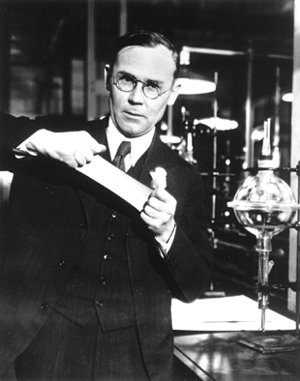
\includegraphics[width=0.24\linewidth]{images/book1/carothers.jpg}

{\small Wallace Carothers dans son laboratoire.}
\end{omfigure}

\section{Structure et propriétés}

Deux échantillons d'un même \omterm{def:g12:polymers:polymer}{polymère} peuvent se comporter très
différemment~: ce qui compte, c'est la longueur des chaînes, leur forme,
et la façon dont elles sont rangées.

\begin{proposition}[Les chaînes et les propriétés]\label{prop:g12:polymers:properties}
\begin{itemize}
  \item Des chaînes plus longues s'enchevêtrent davantage~: le matériau
        est plus résistant et fond à une température plus élevée.
  \item Des chaînes linéaires peuvent s'aligner côte à côte dans des
        régions ordonnées, \emph{cristallines}~; des chaînes ramifiées ne
        le peuvent pas, et restent désordonnées, \emph{amorphes}. Les
        régions cristallines rendent un \omterm{def:g12:polymers:polymer}{polymère} plus dense, plus rigide
        et moins transparent.
  \item Des chaînes maintenues côte à côte par les seules interactions
        intermoléculaires glissent les unes sur les autres quand on les
        chauffe~: le \omterm{def:g12:polymers:polymer}{polymère} est un \omterm{def:g8:plastics:thermoplastic}{thermoplastique}. Des chaînes reliées
        par des \emph{pontages} covalents ne le peuvent pas~: le \omterm{def:g12:polymers:polymer}{polymère}
        est un \omterm{def:g8:plastics:thermoplastic}{thermodurcissable} ou, avec peu de pontages, un solide
        élastique comme le caoutchouc.
\end{itemize}
\end{proposition}

\begin{proof}
Le chauffage donne aux chaînes assez d'énergie pour vaincre les
interactions intermoléculaires qui les unissent
(\cref{ch:g11:polarity-and-cohesion}), plus faibles que les \omterm{def:g10:lewis-and-shape:covalent-bond}{liaisons
covalentes}~; plus les chaînes sont en contact, plus il faut d'énergie.
Les pontages sont covalents~: les rompre détruit le matériau au lieu de
le faire fondre.
\end{proof}

\begin{omfigure}
\begin{tikzpicture}[font=\footnotesize, line width=1pt, line cap=round,
    lab/.style={below, align=center, text width=2.8cm}]
  % linear, packed (crystalline)
  \begin{scope}
    \foreach \y in {0,0.25,0.5,0.75,1.0}
      \draw[omDef] plot[smooth, domain=0:2.2, samples=25] (\x, {\y + 0.05*sin(400*\x)});
    \node[lab] at (1.1,-0.2) {chaînes linéaires\\ alignées~: cristallin};
  \end{scope}
  % linear, tangled (amorphous)
  \begin{scope}[xshift=3.4cm]
    \draw[omDef] plot[smooth] coordinates {(0,0.2) (0.5,0.9) (1.0,0.3) (1.4,1.1) (2.0,0.5) (2.2,0.9)};
    \draw[omProp] plot[smooth] coordinates {(0,0.9) (0.4,0.3) (0.9,1.0) (1.5,0.2) (1.9,1.0) (2.2,0.3)};
    \draw[black!60] plot[smooth] coordinates {(0.1,0.55) (0.7,0.1) (1.2,0.75) (1.7,0.55) (2.2,0.1)};
    \node[lab] at (1.1,-0.2) {chaînes linéaires\\ enchevêtrées~: amorphe};
  \end{scope}
  % branched
  \begin{scope}[xshift=6.8cm]
    \draw[omDef] plot[smooth] coordinates {(0,0.5) (0.6,0.6) (1.2,0.45) (1.8,0.65) (2.2,0.5)};
    \draw[omDef] (0.5,0.6) -- (0.35,1.05) (1.0,0.5) -- (1.15,0.05) (1.6,0.6) -- (1.5,1.1) (1.6,0.6) -- (1.95,1.0);
    \node[lab] at (1.1,-0.2) {chaînes ramifiées~:\\ rangement impossible};
  \end{scope}
  % cross-linked
  \begin{scope}[xshift=10.2cm]
    \foreach \y in {0.1,0.55,1.0}
      \draw[omDef] plot[smooth, domain=0:2.2, samples=25] (\x, {\y + 0.06*sin(300*\x)});
    \foreach \x/\a/\b in {0.4/0.1/0.55, 1.3/0.1/0.55, 0.9/0.55/1.0, 1.9/0.55/1.0}
      \draw[omProp, line width=1.6pt] (\x,\a) -- (\x,\b);
    \node[lab] at (1.1,-0.2) {chaînes pontées~:\\ ne fondent pas};
  \end{scope}
\end{tikzpicture}

{\small Quatre dispositions de chaînes de \omterm{def:g12:polymers:polymer}{polymère}. Les pontages (en
orange) sont des \omterm{def:g10:lewis-and-shape:covalent-bond}{liaisons covalentes} entre chaînes.}
\end{omfigure}

\begin{example}[Deux polyéthylènes]\label{ex:g12:polymers:two-pe}
Le polyéthylène fabriqué sous très haute pression possède de nombreuses
ramifications courtes~: ses chaînes se rangent mal, et il donne des
films souples et transparents pour les sacs. Fabriqué avec un \omterm{def:g12:catalysis:catalyst}{catalyseur}
à basse pression, il a des chaînes presque linéaires, qui se rangent en
régions cristallines~: il est plus dense et plus rigide, et sert à faire
des bouteilles de lait et des caisses. Même \omterm{def:g12:polymers:polymer}{monomère}, même \omterm{def:g12:polymers:repeat-unit}{motif},
architecture différente.
\end{example}

\section{Les polymères naturels}

Les êtres vivants ont fabriqué des \omterm{def:g12:polymers:polymer}{polymères} bien avant les chimistes.

\begin{itemize}
  \item La \textbf{cellulose} et l'\textbf{amidon} sont tous deux des
        chaînes de \omterm{def:g12:polymers:repeat-unit}{motifs} glucose, \ce{C6H10O5} par \omterm{def:g12:polymers:repeat-unit}{motif}, liés
        différemment~: la cellulose forme des fibres droites et
        résistantes (bois, coton, papier)~; l'amidon forme des pelotes
        que l'organisme digère.
  \item Les \textbf{protéines} sont des chaînes d'acides aminés unis par
        des liaisons \omterm{def:g11:functional-groups:amine}{amide}, les liaisons peptidiques du dipeptide du
        \cref{ch:g12:synthesis-strategy}.
  \item L'\textbf{ADN} est une chaîne de nucléotides~; l'ordre de ses
        quatre sortes de \omterm{def:g12:polymers:repeat-unit}{motifs} stocke l'information génétique.
  \item Le \textbf{caoutchouc naturel} est un \omterm{def:g12:polymers:addition-polymer}{polymère d'addition} de
        l'isoprène,
        \ce{CH2=C(CH3)-CH=CH2}, récolté sous forme d'un liquide laiteux, le
        latex, à partir de l'écorce de l'hévéa. Chauffé avec du soufre,
        il voit ses chaînes reliées par des ponts soufrés~: le caoutchouc
        devient plus résistant et garde sa forme, comme dans un pneu.
\end{itemize}

\begin{omfigure}
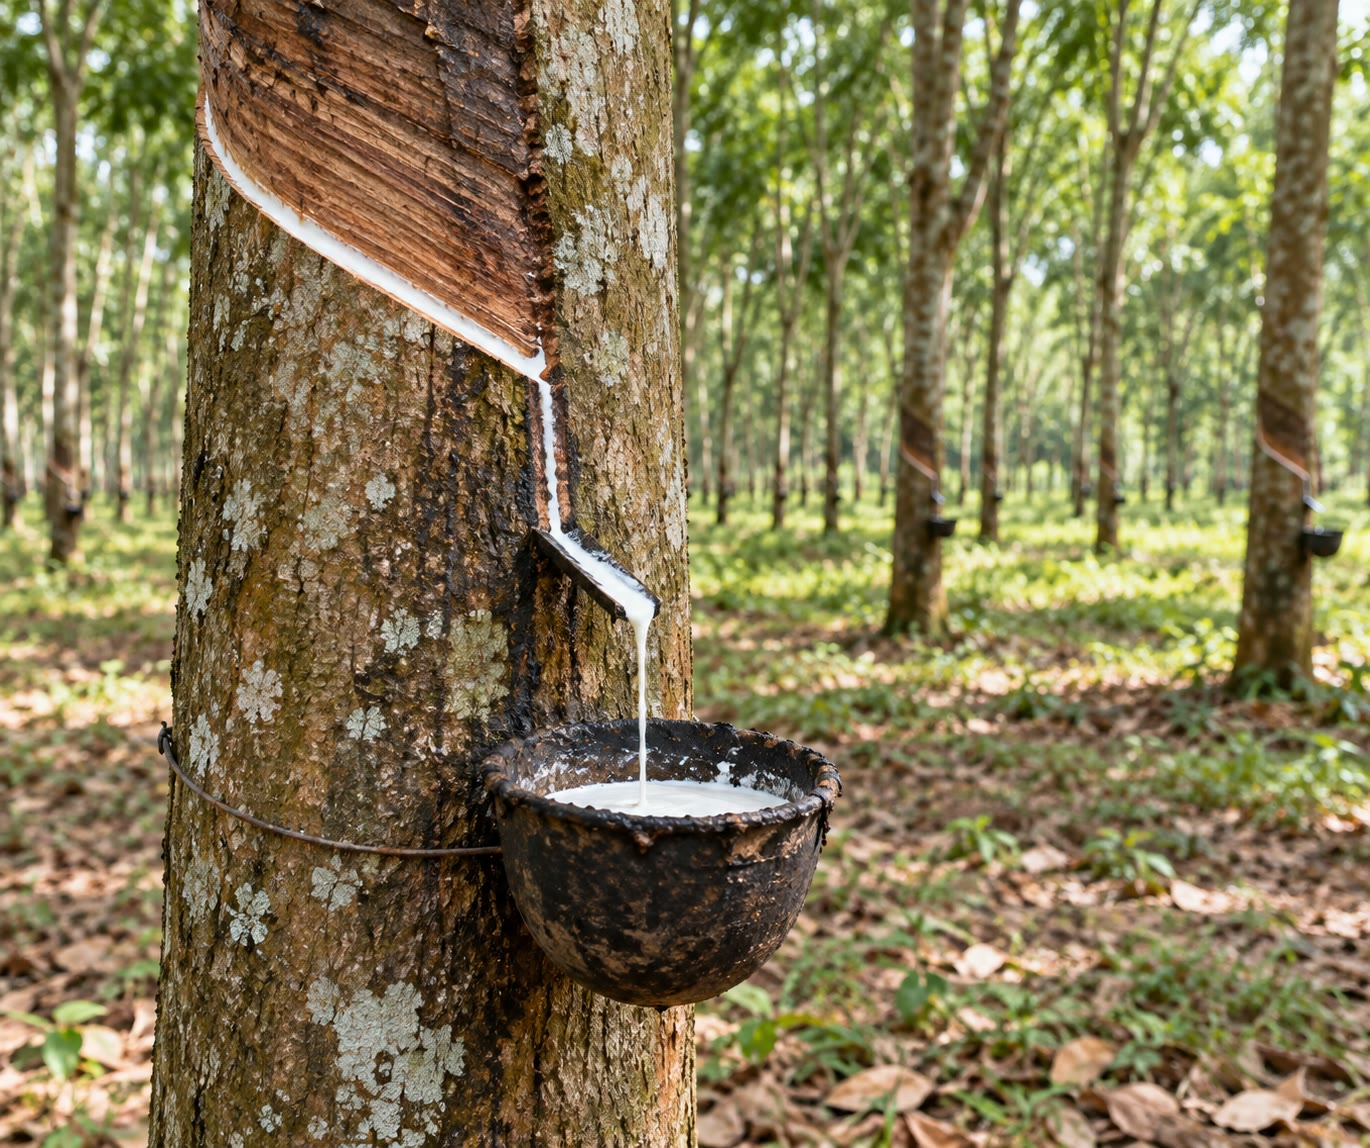
\includegraphics[width=0.45\linewidth]{images/book1/ai/g12-rubber-tapping.jpg}

{\small La saignée d'un hévéa~: le latex s'écoule d'une entaille de
l'écorce dans une coupelle.}
\end{omfigure}

\begin{remark}[Fabriquer et défaire]\label{rem:g12:polymers:recycling}
Un \omterm{def:g8:plastics:thermoplastic}{thermoplastique} peut être fondu et remis en forme~: c'est le
\omterm{def:g5:raw-materials-and-recycling:recycling}{recyclage} mécanique. Un \omterm{def:g12:polymers:addition-polymer}{polymère de condensation} peut aussi être
décomposé en ses \omterm{def:g12:polymers:polymer}{monomères} par la réaction inverse, une hydrolyse, et
les \omterm{def:g12:polymers:polymer}{monomères} transformés en nouveau \omterm{def:g12:polymers:polymer}{polymère}~: c'est le \omterm{def:g5:raw-materials-and-recycling:recycling}{recyclage}
chimique. Un \omterm{def:g8:plastics:thermoplastic}{thermodurcissable} ne se prête facilement ni à l'un ni à
l'autre.
\end{remark}

\section{Exercices}

\begin{exercise}[$\star$]\label{exo:g12:polymers:1}
Donner le \omterm{def:g12:polymers:polymer}{monomère} du polypropylène, dont le \omterm{def:g12:polymers:repeat-unit}{motif} est
\ce{-CH2-CH(CH3)-}.
\end{exercise}

\begin{exercise}[$\star$]\label{exo:g12:polymers:2}
Écrire le \omterm{def:g12:polymers:repeat-unit}{motif} du \omterm{def:g12:polymers:polymer}{polymère} fabriqué à partir du tétrafluoroéthène,
\ce{CF2=CF2}. Est-ce un \omterm{def:g12:polymers:addition-polymer}{polymère d'addition} ou de condensation~?
\end{exercise}

\begin{exercise}[$\star$]\label{exo:g12:polymers:3}
Classer en \omterm{def:g12:polymers:addition-polymer}{polymères d'addition} ou de condensation~: le polyéthylène,
le PET, le nylon, le PVC, le polystyrène.
\end{exercise}

\begin{exercise}[$\star$]\label{exo:g12:polymers:4}
Lesquels de ces \omterm{def:g12:polymers:polymer}{polymères} sont naturels~: la cellulose, le nylon,
l'amidon, le PVC, le caoutchouc issu du latex, les protéines~?
\end{exercise}

\begin{exercise}[$\star$]\label{exo:g12:polymers:5}
Pourquoi chaque \omterm{def:g12:polymers:polymer}{monomère} d'un \omterm{def:g12:polymers:addition-polymer}{polymère de condensation} doit-il porter
deux groupes \omterm{def:g7:chemical-reactions:reactant}{réactifs}~?
\end{exercise}

\begin{exercise}[$\star\star$]\label{exo:g12:polymers:6}
Un échantillon de PVC a une \omterm{def:g10:the-mole:molar-mass}{masse molaire} moyenne de
\qty{125000}{g/mol}. Calculer son \omterm{def:g12:polymers:repeat-unit}{degré de polymérisation}.
\end{exercise}

\begin{exercise}[$\star\star$]\label{exo:g12:polymers:7}
Une chaîne de polystyrène a un \omterm{def:g12:polymers:repeat-unit}{degré de polymérisation} de 2500.
Calculer sa \omterm{def:g10:the-mole:molar-mass}{masse molaire}.
\end{exercise}

\begin{exercise}[$\star\star$]\label{exo:g12:polymers:8}
L'acide lactique, \ce{CH3-CH(OH)-COOH}, porte un groupe \omterm{def:g11:functional-groups:alcohol}{alcool} et un
groupe acide. Montrer qu'il peut former à lui seul un polyester, écrire
son \omterm{def:g12:polymers:repeat-unit}{motif}, et nommer la petite \omterm{def:g7:atoms-and-molecules:molecule}{molécule} libérée.
\end{exercise}

\begin{exercise}[$\star\star$]\label{exo:g12:polymers:9}
Expliquer, à l'aide de la figure des dispositions de chaînes, pourquoi
les films pour sacs sont souples et transparents alors que les
bouteilles de lait sont rigides et opaques.
\end{exercise}

\begin{exercise}[$\star\star$]\label{exo:g12:polymers:10}
Le manche d'une casserole est en \omterm{def:g8:plastics:thermoplastic}{thermodurcissable}, le bouton en
plastique de son couvercle aussi. Décrire leurs chaînes. Pourquoi ne
peut-on pas les fondre et les recycler~?
\end{exercise}

\begin{exercise}[$\star\star$]\label{exo:g12:polymers:11}
Une chaîne de nylon-6,6 a une \omterm{def:g10:the-mole:molar-mass}{masse molaire} de \qty{22600}{g/mol}.
Calculer la \omterm{def:g10:the-mole:molar-mass}{masse molaire} de son \omterm{def:g12:polymers:repeat-unit}{motif} \ce{C12H22N2O2}, puis son \omterm{def:g12:polymers:repeat-unit}{degré
de polymérisation}.
\end{exercise}

\begin{exercise}[$\star\star\star$]\label{exo:g12:polymers:12}
Écrire la réaction entre une \omterm{def:g7:atoms-and-molecules:molecule}{molécule} d'hexane-1,6-diamine et une
\omterm{def:g7:atoms-and-molecules:molecule}{molécule} d'acide hexanedioïque, qui donne la première liaison \omterm{def:g11:functional-groups:amine}{amide}.
Pourquoi le produit peut-il continuer à réagir par ses deux
extrémités~?
\end{exercise}

\begin{exercise}[$\star\star\star$]\label{exo:g12:polymers:13}
Quelle masse d'eau est libérée lors de la fabrication de \qty{1.0}{kg}
de nylon-6,6~?
\end{exercise}

\begin{exercise}[$\star\star\star$]\label{exo:g12:polymers:14}
Le caoutchouc naturel est mou et collant quand il est chaud~; chauffé
avec du soufre, il devient le caoutchouc élastique et résistant des
pneus. Expliquer à l'aide des chaînes. Pourquoi un pneu est-il si
difficile à recycler~?
\end{exercise}

\begin{exercise}[$\star\star\star$]\label{exo:g12:polymers:15}
L'amidon et la cellulose ont la même formule par \omterm{def:g12:polymers:repeat-unit}{motif}, \ce{C6H10O5}.
Une chaîne de cellulose a une \omterm{def:g10:the-mole:molar-mass}{masse molaire} de \qty{1.6e6}{g/mol}.
Combien de \omterm{def:g12:polymers:repeat-unit}{motifs} glucose contient-elle~? Quelle est sa longueur, si
chaque \omterm{def:g12:polymers:repeat-unit}{motif} ajoute \qty{0.5}{nm} à sa longueur~?
\end{exercise}

\section{Problème~: de la bouteille à la veste polaire}

\begin{problem}[{Problème du week-end --- combien de bouteilles de
25~g faut-il pour une veste polaire~?}]
\label{pb:g12:polymers:1}
% ledger: aw:C, aw:H, aw:O
Une veste polaire est faite de \qty{300}{g} de fibre de PET. On collecte
des bouteilles usagées de
\qty{25}{g} chacune, qui sont triées, lavées, broyées, fondues et
filées~; au cours de ce procédé, \qty{80}{\percent} de la masse des
bouteilles se retrouve sous forme de fibre dans la veste.

\medskip
\noindent\textbf{Partie I --- Le \omterm{def:g12:polymers:polymer}{polymère}.}
\begin{enumerate}
  \item Nommer les deux \omterm{def:g12:polymers:polymer}{monomères} du PET et les \omterm{def:g11:functional-groups:functional-group}{groupes caractéristiques}
        qu'ils portent.
  \item Quelle liaison se forme entre eux~? Quelle petite \omterm{def:g7:atoms-and-molecules:molecule}{molécule} est
        libérée~?
  \item Le PET est-il un \omterm{def:g12:polymers:addition-polymer}{polymère d'addition} ou de condensation~?
  \item Calculer les \omterm{def:g10:the-mole:molar-mass}{masses molaires} des deux \omterm{def:g12:polymers:polymer}{monomères}.
  \item En déduire la \omterm{def:g10:the-mole:molar-mass}{masse molaire} du \omterm{def:g12:polymers:repeat-unit}{motif} \ce{C10H8O4}, et la
        vérifier à l'aide de sa formule.
\end{enumerate}

\medskip
\noindent\textbf{Partie II --- Les chaînes.}
\begin{enumerate}[resume]
  \item Le PET d'une bouteille a des chaînes de \omterm{def:g10:the-mole:molar-mass}{masse molaire} moyenne
        \qty{38400}{g/mol}. Calculer le \omterm{def:g12:polymers:repeat-unit}{degré de polymérisation}.
  \item Combien de liaisons \omterm{def:g11:functional-groups:carboxylic-acid}{ester} une chaîne contient-elle, environ~?
  \item Le PET des bouteilles est en partie cristallin. Qu'est-ce que
        cela indique sur ses chaînes~?
  \item Pourquoi peut-on fondre le PET et le filer en fibre~?
\end{enumerate}

\medskip
\noindent\textbf{Partie III --- Le \omterm{def:g5:raw-materials-and-recycling:recycling}{recyclage}.}
\begin{enumerate}[resume]
  \item Quelle masse de bouteilles faut-il pour une veste~?
  \item Combien de bouteilles cela représente-t-il~?
  \item Que devient le reste de la masse~?
  \item Quel principe de la \omterm{def:g12:synthesis-strategy:green-chemistry}{chimie verte} ce \omterm{def:g5:raw-materials-and-recycling:recycling}{recyclage} applique-t-il~?
\end{enumerate}

\medskip
\noindent\textbf{Partie IV --- Retour aux \omterm{def:g12:polymers:polymer}{monomères}.}
\begin{enumerate}[resume]
  \item Écrire, pour un \omterm{def:g12:polymers:repeat-unit}{motif}, l'hydrolyse du PET en ses \omterm{def:g12:polymers:polymer}{monomères}.
  \item Quelle quantité de \omterm{def:g12:polymers:repeat-unit}{motifs} y a-t-il dans \qty{1.00}{kg} de PET~?
  \item Quelles masses de chacun des \omterm{def:g12:polymers:polymer}{monomères} l'hydrolyse complète de
        \qty{1.00}{kg} de PET donne-t-elle~?
  \item Quelle masse d'eau consomme-t-elle~? Vérifier la \omterm{def:g8:balanced-equations:conservation}{conservation
        de la masse}.
  \item Donner un avantage de ce \omterm{def:g5:raw-materials-and-recycling:recycling}{recyclage} chimique par rapport à la
        fusion.
  \item Donner la réponse finale~: combien de bouteilles de \qty{25}{g}
        faut-il pour une veste polaire~?
\end{enumerate}
\end{problem}
